\section{Studying Shortest Paths}
\label{sec:stats}

In \nameref{prob:shortest-path} we are given a query $(s, t)$, the source and target vertices, as well as the realised cost function $c \sim \mathcal D$. The difficulty of returning a short path from $s$ to $t$ varies greatly upon the vertex pair and $\mathcal D$. Possibly, $t$ is reachable from $s$ only with a singular path, or there is one path $P^*$, such that for any $c\in\mathcal C$ the cost $f_c(P^*)$ is cheapest possible cost of reaching $t$ from $s$. In such cases, if we find that path we can be sure we always return it no matter the realisation of $c$, and the answers are even optimal.

On the other hand, we can easily construct arbitrarily hard graphs and queries. For some pair $(s, t)$ in $V$, there can be $\mathcal O(n!)$ many paths that connect them, and for each such $P$ we could assign exactly one cost function in $\mathcal C$ where any other path $P'$ costs arbitrarily much more; $f_c(P') > z\cdot f_c(P)$ for any $z \in \mathbb R$. For such a difficult setting the portfolio method will be unusable, the probability that a cheap path is in the portfolio would be $O(1 / n!)$. In such settings it is prudent to pay in query time and use \cref{alg:dijkstra}. Real-world traffic networks are not very likely to behave this way, and that is the point we want to make use of.

Hence, we study the $(s,t)$-pairs in \cref{shanghai} and \cref{losangeles} in order to better grasp the structure of their graphs and cost distributions.
For that purpose let us find patterns of the distance random variables $d_{s,t}$ for all $s, t$. \Cref{shanghai_hist} shows the expected distance over the vertex pairs in \cref{shanghai}.

\begin{figure}
    \centering
    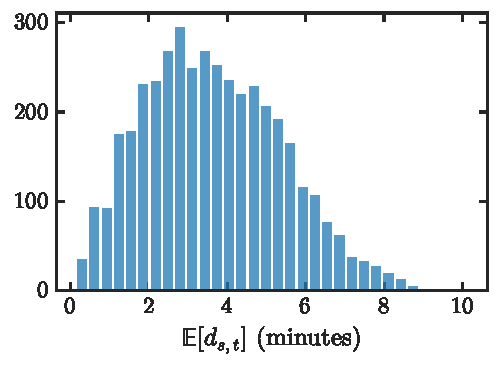
\includegraphics{figures/sh_hist.pdf}
    \caption{Histogram of the expected distance between all $(s, t)$ pairs, where $t$ is reachable $s$ in \cref{shanghai}.}
    \label{fig:shanghai_hist}
\end{figure}

We see there is a wide range of average distances. This is intuitive, shortest path costs should vary greatly for vertices sharing their neighbourhood in comparison to vertices on opposite ends of the entire graph. With similar intuition, we could claim that \nameref{prob:shortest-path} decreases in difficulty for $(s,t)$ that are adjacent in the graph. For ``behaved'' distributions $\mathcal D$ there might not by any scenarios, where the direct path using the edge $(s,t)$ is not the most sensible answer.

In order to find some first $(s,t)$-queries that should prove interesting or difficult, we use scatter plots in the following discussion of $(s, t)$ pairs. There, each marker is two-coloured, indicating the values of $s$ and $t$ respectively. Let us first plot the already shown $\mathbb{E}[d_{s,t}]$ against the standard deviation of those same random variables, $\sigma(d_{s,t})$.

\begin{figure}
    \centering
    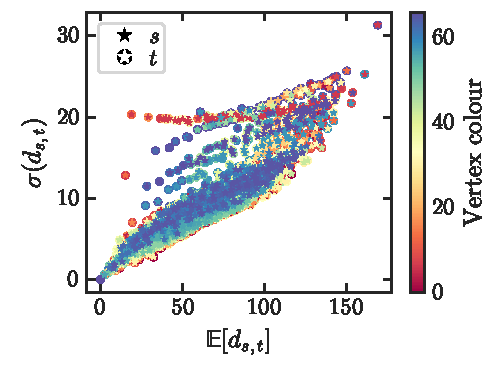
\includegraphics{figures/sh_mean_std.pdf}
\caption{The expectance values against the standard deviation of $d_{s,t}$ over all $(s, t)$ pairs in \cref{shanghai}. Each point corresponding to an $(s,t)$ pair is two-coloured matching the colouring in \cref{fig:shanghai} in order to more easily find the corresponding pairs there. For a larger, interactive plot visit \href{https://finnharbeke.github.io/shortest-path-portfolios/sh_dist_scatter.html}{this project’s GitHub Pages}.}
\label{fig:mean_vs_std}
\end{figure}

Clearly, the expected distance and the standard deviation are very correlated and most points in the plot are found in one big cloud. Interestingly, one can find these strings of points with similar colours that form lines. Upon further inspection we notice that they form pairs of vertices with shared commonly used subpaths. Noteworthy are the $(6, 66)$ vertex pair, that is the pair with the furthest average travel distance as well as the highest absolute standard deviation. As well as $(6, 13)$, for which the ratio of standard deviation over expected value is the highest. Note $(6, 13)$ is an edge in \cref{shanghai}, as well as the only path from $6$ to $13$, and it influences the entirety of the red band that is dotted almost horizontally along the grid line of a standard deviation of 20, which are all pairs whose source is $6$.

This observation plays into the discussion of the difficulty of a source-target pair very crucially. $(6, 13)$ is not a difficult pair, there is only one single path to reach $13$ from $6$. The high variance of a single edge in the graph does not imply that many different paths are the shortest in distinct events from the distribution. Instead, let us consider a new measure of uncertainty given $(s, t)$.

The shortest path's \emph{entropy} is
\[
H(P^*_{s,t}) = -\sum_{P \in \mathcal{P}_{s,t}} \Pr(P^*_{s,t} = P) \log \Pr(P^*_{s,t} = P),
\]
with the convention that $0 \log 0 = 0$. The entropy measures the uncertainty in which path will be the shortest.

Think of $P^*_{s,t}$ as a categorical random variable taking values like ``along the lake'' or ``the highway'', indicating which path is best as of now. When it is clear that the path is the same for all cost functions $c \in \mathcal C$, then \nameref{prob:shortest-path} is trivial, a portfolio of size $1$ is optimal and we always return that path. But when it takes many different values in many different events, that is when things become more difficult. The entropy of the shortest path should capture a notion that is related to the difficulty of the query $(s,t)$. Thus, we plot $H(P^*_{s,t})$ for all $s, t$ in \cref{fig:entropy_std}, in comparison the already discussed $\sigma(d_{s,t})$.

\begin{figure}
    \centering
    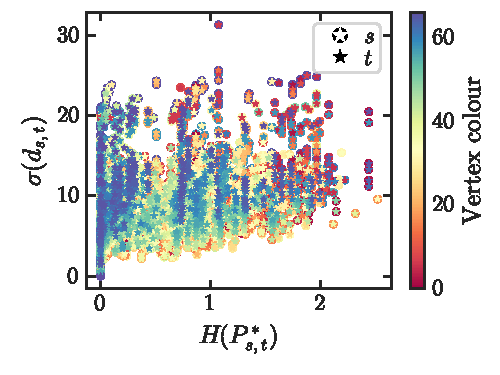
\includegraphics{figures/sh_entropy_std.pdf}
    \caption{The entropy of the shortest path against the standard deviation of $d_{s,t}$ over all $(s, t)$ pairs in \cref{shanghai}. Each point corresponding to an $(s,t)$ pair is two-coloured matching the colouring in \cref{fig:shanghai} in order to more easily find the corresponding pairs there. For a larger, interactive plot visit \href{https://finnharbeke.github.io/shortest-path-portfolios/sh_entr_std_scatter.html}{this project’s GitHub Pages}.}
    \label{fig:entropy_std}
\end{figure}

We're quick to see how different of a picture the shortest path entropy paints in comparison to the standard deviation of the distance. The perfectly vertical strings of points are pairs that share subpaths, and because they have the same entropy they must be using the same subpaths in the exact same events. It is only the edges that are appended to the ends of those subpaths for some pairs that change the standard deviation of the distance considerably.

In essence the entropy describes the uncertainty of what path will be the shortest. With less entropy, it thus is more likely that the shortest path is one that we expect. 


